\section{Database}
To support the necessary information storage, a database is implemented in accordance with the ER diagram described in \secref{sec:ERdiagram}.
The implementation of the ER diagram leads to the database schema that can be seen in \figref{fig:Database-tables}, however, there is more than what the ER diagram describes.
In this figure, the connections between the tables represents foreign key constraints.

\begin{figure}[h]
	\centering
	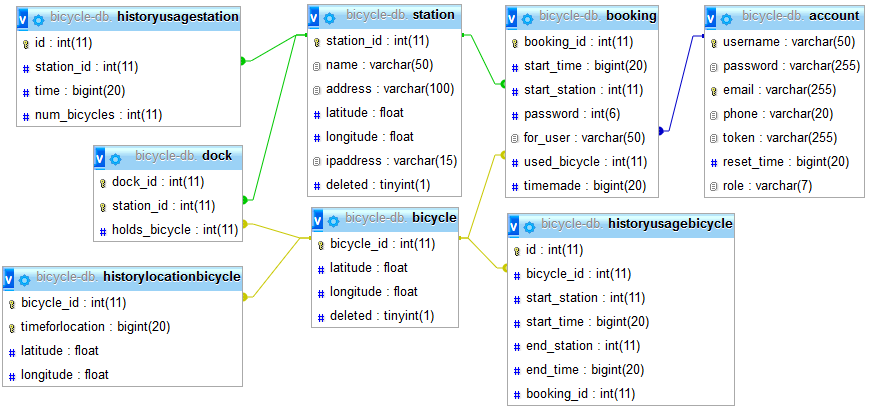
\includegraphics[scale=0.6]{Database/DBtables}
	\caption{Database tables, foreign keys represented with the colours green for \texttt{station_id}, yellow for \texttt{bicycle_id}, and blue for \texttt{username}.}\label{fig:Database-tables}
\end{figure}

The additional tables (\texttt{history\-usage\-station}, \texttt{history\-usage\-bicycle}, and \texttt{history\-lo\-ca\-ti\-on\-bi\-cy\-cle}) are added to store the information needed for the features described in \secref{sec:designAdminTools} and which implementation is discussed in \secref{sec:impAdminTools}.
The three additional tables serves as a log, in order to store information about usage of the system, used by the administration part of the system to analyse on the usage of the system.

Logging is different from the general usage of the system in that it uses all historical data.
That means for the purposes of the tables mentioned above it is important for the station and bicycle tables that rows are not deleted, but rather flagged as deleted, which is the cause of the deleted attribute in those tables. 
For regular use of the system it changes little but administratively it allows for using historical data.

In the translation from the ER diagram to the schema presented, the relations between the various entities could in all cases be represented as an attribute on one of the involved entities, as no N to M relations exist.
This was all that was needed to convert the ER diagram into the database schema, however, with the introduction of the administrator features and their associated data tables, more was needed.

When the administrator features was added into the database, in addition to adding three new tables to contain their information.
The administrator features also required additional attributes to some of the already existing tables, an example of this being \texttt{role} attribute on the \texttt{account} table, used to distinguish regular users from the ones with administrator privileges.

This was implemented in MySQL \citep{misc:mysql}, primarily because it was packaged with the webserver that we used to develop the system with.
There is no reason why MySQL was chosen instead of competing DBMS such as postgresql \citep{misc:postgres} or MSSQL \citep{misc:mssql} other than convenience, and little reason why the schema could not be adapted to work on others. 